\chapter{Preliminares}

En este capítulo presentaremos las herramientas básicas para el desarrollo del resultado principal de este Trabajo Fin de Grado: El teorema de Radó. Para ello necesitaremos el concepto de curva de Jordan, amén del teorema del mismo nombre y de su generalización, el teorema de Jordan-Schönflies. En la siguiente sección introduciremos el lenguaje que necesitaremos para la demostración de estos resultados, enfatizando el teorema de la curva de Jordan. El teorema de Jordan-Schönflies se enunciará sin demostración porque su tratamiento queda lejos de las competencias dadas a este trabajo.

\section{Teorema de la curva de Jordan}

Comencemos con la idea básica de una curva cerrada en el plano que sin autointersecciones, esto es, una circunferencia.

Es fácil ver   que  ésta divide en dos partes el plano. Como muchos otros resultados en Matemáticas que a simple vista parecen sencillos, probar que toda curva cerrada sin autointersecciones divide en dos partes el plano no es tarea fácil.

Este será el resultado que desarrollaremos en éste apartado, para el que necesitaremos del lenguaje topológico apropiado que introducimos a continuación.

\subsection{Conceptos básicos de Topología}

\begin{definition}
	Un espacio topológico es un par ($X$,$\tau$) donde
	\begin{enumerate}
		\item  $X$ es un conjunto no vacío.
		\item $\tau \subseteq \mathit{P}(X)$
	\end{enumerate}
	satisfaciendo:
	\begin{enumerate}
		\item $\emptyset \text{,} X \in \tau$
		\item Si $O_1 \text{,} O_2 \in \tau \Longrightarrow O_1 \bigcap O_2 \in \tau$
		\item Si $\{ O_\lambda \text{, } \lambda \in \Lambda \} \subseteq \tau \Longrightarrow \bigcup_{\lambda \in \Lambda} O_\lambda \in \tau$
	\end{enumerate}
\end{definition}


\begin{definition}
	Sean $X$ e $Y$ dos espacios topológicos y $f$ una función de $X$ en $Y$; $f$ se dice un homeomorfismo si, y sólo si, cumple las siguientes condiciones:
	\begin{enumerate}
		\item $f$ es biyectiva.
		\item $f$ es continua.
		\item La inversa de $f$ es continua.
	\end{enumerate}
\end{definition}

Si $f : X \rightarrow Y$ es un homeomorfismo, $X$ se dice homeomorfo a $Y$. Además conservan los llamados invariantes topológicos.

Ejemplos claros de homeomorfismos:

\begin{enumerate}
	\item La circunferencia menos un punto es homeomorfa a la recta real. El homeomorfismo definido sería la conocida como proyección estereográfica.
	\item Un cono sin el vértice es homeomorfo a un cilindro.
\end{enumerate}

\begin{definition}
	Un arco en un espacio topológico ($X$,$\tau$) es un aplicación continua $\alpha: I\subset \mathbb{R} \rightarrow (X,\tau)$, donde $I = [a,b] \hspace{0.2cm} \text{, con } a \textless b$, dotado de la topología euclídea.
\end{definition}

Al conjunto $\gamma = \{ \alpha(t) : t \in I \}$ se le llamará traza del arco $\alpha$.

Éste concepto se extiende de forma natural a arcos abiertos definidos en todo $\mathbb{R}$, aunque nosotros nos centraremos a curvas definidas en intervalos de la forma $[a,b]$ como en la definición. Los puntos  $\alpha(a)$ y $\alpha(b)$ se referirán como el inicio y el final de la arco $\alpha$, respectivamente, y también se dirá que éste une $\alpha(a)$ y $\alpha(b)$.

\begin{definition}
	Un arco $\alpha$ se dirá cerrado si sus extremos coinciden, es decir, si $\alpha(a) = \alpha(b)$.
\end{definition}

\begin{definition}
	Una arco $\alpha\colon [a,b]\to X$ se dirá de Jordan si no se autointersecta a sí mismo, esto es:\[\ \alpha(t_1) \neq \alpha(t_2) \hspace{0.5cm}\forall \hspace{0.1cm}t_1,t_2 \in [a,b] \]
En otras palabras, $\alpha$ es de Jordan  si la aplicación $\alpha$ es inyectiva.
\end{definition}



\begin{definition}
	Una curva $\alpha : [a,b] \rightarrow X$ es de Jordan si es un arco cerrado tal que $\alpha \vert_{[a,b[}$ es inyectiva. Equivalentemente, una aplicación continua $\alpha : \mathbb{S}^1 \rightarrow X$ sin autointersecciones.
\end{definition}

\begin{definition}
	Decimos que un espacio topológico ($X$,$\tau$) es arcoconexo, si cualesquiera dos puntos de $X$ están unidos por un arco.
\end{definition}

\begin{definition}
	Un arco poligonal simple (o una curva de Jordan poligonal, si es cerrado) en $\mathbb{R}^2$ con la topología euclídea es un arco simple (o curva de Jordan, si es cerrado) cuya traza es  unión finita de segmentos.
\end{definition}

\begin{lemma}
	Sea $\Omega$ un conjunto abierto conexo del plano, entonces cualesquiera dos puntos en $\Omega$ se pueden unir por un arco poligonal simple en $\Omega$. 
\end{lemma}

\begin{definition}
	Una componente conexa de un espacio topológico es un subespacio topológico conexo maximal. Un espacio topológico se dice localmente conexo (arcoconexo) si todo punto admite una base de entornos conexos (arcoconexos). 
\end{definition}
\begin{lemma}
Todo espacio topológico conexo y localmente arcoconexo es arcoconexo. Como todo abierto del plano es localmente arcoconexo (de hecho, localmente {\em poligonalmente conexo}), las componentes conexas de un abierto del plano son poligonalmente conexas. 
\end{lemma}

\subsection{Teoría básica de grafos}

Una vez presentado el lenguaje topológico necesario para el desarrollo de nuestro tema, introduciremos a continuación la teoría básica de grafos. Ésta nos ayudará a demostrar el teorema de la curva de Jordan, meta principal de este apartado.

\begin{definition}
	Un grafo G es la unión de dos conjuntos disjuntos $V(G)$ y $E(G)$, llamado vértices y aristas respectivamente, tal que para cada arista existen asociados dos vértices distintos $x$ e $y$, llamados extremos de la arista.
\end{definition}



\begin{definition}
	Diremos que dos vértices $u$ y $v$ de un grafo $G$ son adyacentes si, y sólo si, están unidos por una arista.
\end{definition}

A partir de ahora  nos restringiremos a grafos  satisfaciendo la siguiente propiedad: 
\begin{quote} {\em Si dos vértices $x$ e $y$   son adyacentes entonces hay una única arista que los une, que denotaremos $xy$.}
\end{quote}
Por tanto no cabe confusión al nombrar las aristas en función de sus vértices.

\begin{definition}
	Se define un isomorfismo de grafos $G$ y $H$ como una función biyectiva $f : V(G) \rightarrow V(H)$ que preserva la relación de adyacencia. Es decir, un par de vértices $u$ y $v$ de $G$ son adyacentes si, y sólo si, $f(u)$ y $f(v)$ son adyacentes en $H$.
\end{definition}

Por ejemplo los siguientes grafos son isomorfos:
\[\]
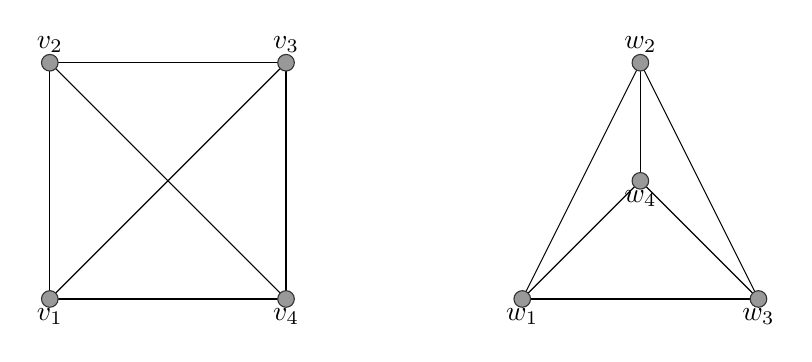
\begin{tikzpicture}[y=.3cm, x=.3cm,font=\normalsize]
\draw (0,0) -- (10,10);
\draw (0,0) -- (0,10);
\draw (0,0) -- (10,0);
\draw (10,0) -- (10,10);
\draw (10,0) -- (0,10);
\draw (0,10) -- (10,10);

\filldraw[fill=black!40,draw=black!80] (0,0) circle (3pt)    node[anchor=north] {$v_1$};
\filldraw[fill=black!40,draw=black!80] (0,10) circle (3pt)    node[anchor=south] {$v_2$};
\filldraw[fill=black!40,draw=black!80] (10,10) circle (3pt)    node[anchor=south] {$v_3$};
\filldraw[fill=black!40,draw=black!80] (10,0) circle (3pt)    node[anchor=north] {$v_4$};

\draw (20,0) -- (25,10);
\draw (20,0) -- (25,5);
\draw (20,0) -- (30,0);
\draw (30,0) -- (25,10);
\draw (30,0) -- (25,5);
\draw (25,10) -- (25,5);

\filldraw[fill=black!40,draw=black!80] (20,0) circle (3pt)    node[anchor=north] {$w_1$};
\filldraw[fill=black!40,draw=black!80] (25,10) circle (3pt)    node[anchor=south] {$w_2$};
\filldraw[fill=black!40,draw=black!80] (30,0) circle (3pt)    node[anchor=north] {$w_3$};
\filldraw[fill=black!40,draw=black!80] (25,5) circle (3pt)    node[anchor=north] {$w_4$};
\end{tikzpicture}
\[\]
	El isomorfismo se define para como el único que lleva $v_{i}$ en $w_{i}$ $\forall i = 1,2,3,4$.

\begin{definition}
Un camino es un grafo con vértices $v_{1},...,v_{n}$ y aristas $v_{1},v_{2},...,v_{n-1}v_{n}$. Denotaremos un camino por $v_{1}v_{2}...v_{n}$.

Si además $n \geq 3$ y añadimos una arista $v_{n}v_{1}$ a un camino dado obtenemos un camino cerrado al que llamaremos ciclo y denotaremos por $C_n$.
\end{definition}

	A continuación tenemos un ejemplo sencillo de un camino con 4 vértices y un ciclo con 4 vértices también, a los que denominaremos $v_{1}v_{2}v_{3}v_{4}$ y $C_4$ por la notación que hemos convenido:
\[\]
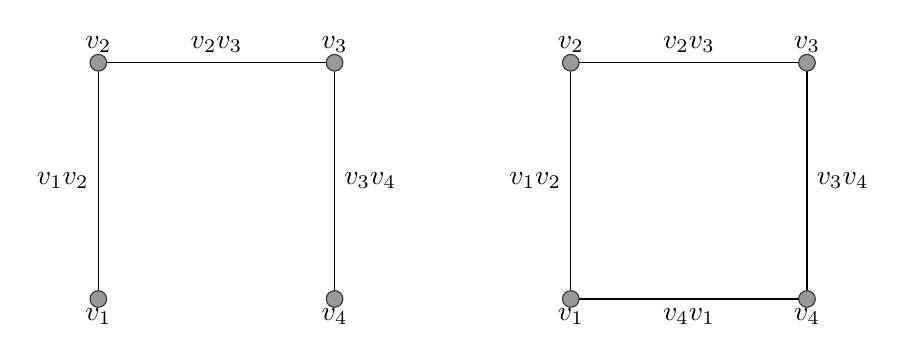
\begin{tikzpicture}[y=.3cm, x=.3cm,font=\normalsize]
\draw (0,0) -- (0,10);
\draw (10,0) -- (10,10);
\draw (10,10) -- (0,10);

\filldraw[fill=black!40,draw=black!80] (0,0) circle (3pt)    node[anchor=north] {$v_1$};
\filldraw[fill=black!40,draw=black!80] (0,10) circle (3pt)    node[anchor=south] {$v_2$};
\filldraw[fill=black!40,draw=black!80] (10,10) circle (3pt)    node[anchor=south] {$v_3$};
\filldraw[fill=black!40,draw=black!80] (10,0) circle (3pt)    node[anchor=north] {$v_4$};

\node [above] at (5,10) {$v_{2}v_{3}$};
\node [right] at (10,5) {$v_{3}v_{4}$};
\node [left] at (0,5) {$v_{1}v_{2}$};

\draw (20,0) -- (20,10);
\draw (30,0) -- (30,10);
\draw (30,10) -- (20,10);
\draw (20,0) -- (30,0);

\filldraw[fill=black!40,draw=black!80] (20,0) circle (3pt)    node[anchor=north] {$v_1$};
\filldraw[fill=black!40,draw=black!80] (20,10) circle (3pt)    node[anchor=south] {$v_2$};
\filldraw[fill=black!40,draw=black!80] (30,10) circle (3pt)    node[anchor=south] {$v_3$};
\filldraw[fill=black!40,draw=black!80] (30,0) circle (3pt)    node[anchor=north] {$v_4$};

\node [above] at (25,10) {$v_{2}v_{3}$};
\node [right] at (30,5) {$v_{3}v_{4}$};
\node [left] at (20,5) {$v_{1}v_{2}$};
\node [below] at (25,0) {$v_{4}v_{1}$};
\end{tikzpicture}
\[\]
	Si $G$ es un grafo y $A \subseteq V(G) \cup E(G)$, entonces $G - A$ es el grafo obtenido de $G$ al eliminar todos los vértices y aristas que pertenezcan a $A$,  y todas las aristas  de $G$ incidentes en un vértice de $A$ (aunque no pertenezcan a  $A$).

	Veamos un ejemplo gráfico:
\[\]
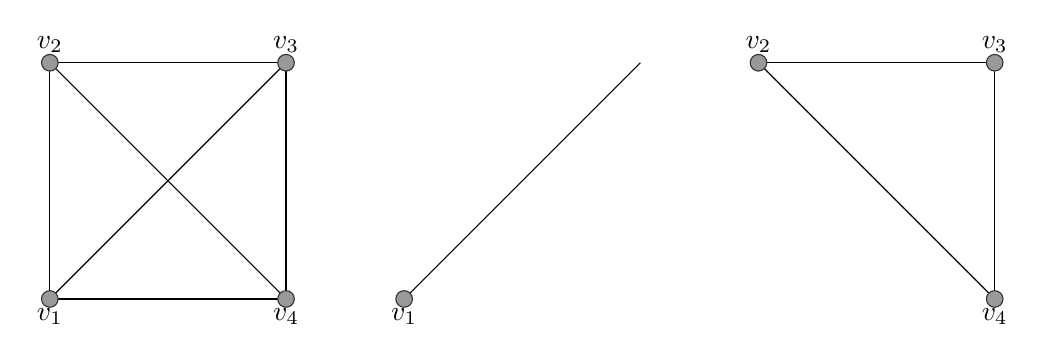
\begin{tikzpicture}[y=.3cm, x=.3cm,font=\normalsize]
\draw (0,0) -- (10,10);
\draw (0,0) -- (0,10);
\draw (0,0) -- (10,0);
\draw (10,0) -- (10,10);
\draw (10,0) -- (0,10);
\draw (0,10) -- (10,10);

\filldraw[fill=black!40,draw=black!80] (0,0) circle (3pt)    node[anchor=north] {$v_1$};
\filldraw[fill=black!40,draw=black!80] (0,10) circle (3pt)    node[anchor=south] {$v_2$};
\filldraw[fill=black!40,draw=black!80] (10,10) circle (3pt)    node[anchor=south] {$v_3$};
\filldraw[fill=black!40,draw=black!80] (10,0) circle (3pt)    node[anchor=north] {$v_4$};


\draw (15,0) -- (25,10);

\filldraw[fill=black!40,draw=black!80] (15,0) circle (3pt)    node[anchor=north] {$v_1$};

\draw (40,0) -- (40,10);
\draw (40,0) -- (30,10);
\draw (30,10) -- (40,10);

\filldraw[fill=black!40,draw=black!80] (30,10) circle (3pt)    node[anchor=south] {$v_2$};
\filldraw[fill=black!40,draw=black!80] (40,10) circle (3pt)    node[anchor=south] {$v_3$};
\filldraw[fill=black!40,draw=black!80] (40,0) circle (3pt)    node[anchor=north] {$v_4$};
\end{tikzpicture}
\[\]
En este ejemplo tan simple, el grafo de la izquierda sería nuestro grafo $G$, la figura central es lo que hemos llamado $A$ y, finalmente, el grafo de la derecha sería $G-A$.

\begin{definition}
	Decimos que un grafo $G$ es conexo si para cada par de vértices $u$ y $v$ en $G$ se puede encontrar un camino en $G$ que los una.
\end{definition}

\begin{definition}
	Decimos que un grafo $G$ es biconexo si es conexo y para vértice $v$ en $G$, $G - \{v\}$ (que también podremos denotar como $G - v$) es conexo.
\end{definition}

\begin{definition}
Un grafo $G$ se dice que puede ser embebido en un espacio topológico $X$ si los vértices de $G$ pueden ser representados por puntos distintos de $X$ y cada arista de $G$ puede ser representada como un arco de Jordan en X uniendo los puntos que representan a sus vértices, de  modo que dos aristas distintas se cortan a lo más un extremo en común.
\end{definition}

\begin{definition}
Los  grafos abstractos que pueden ser embebidos en $\mathbb{R}^2$ se dirán planos.
\end{definition}

En muchas ocasiones no haremos distinción entre un grafo abstracto plano y el grafo euclidiano asociado   a su representación (o dibujo) en $\mathbb{R}^2$ mediante puntos y arcos. Veamos algunos ejemplos:

\[\]
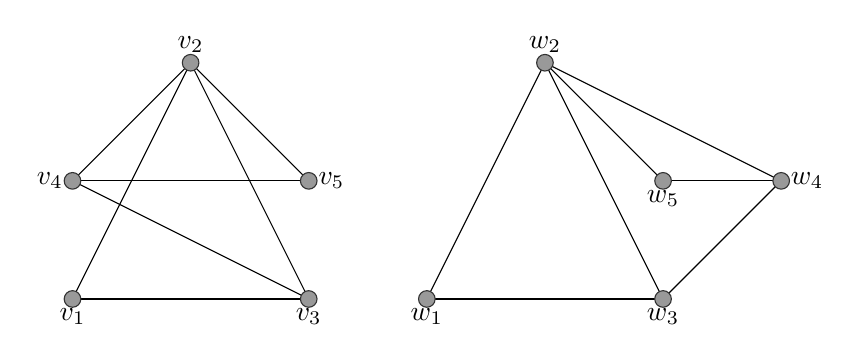
\begin{tikzpicture}[y=.3cm, x=.3cm,font=\normalsize]

\draw (0,0) -- (5,10);
\draw (0,0) -- (10,0);
\draw (10,0) -- (5,10);
\draw (10,0) -- (0,5);
\draw (0,5) -- (10,5);
\draw (0,5) -- (5,10);
\draw (10,5) -- (5,10);

\filldraw[fill=black!40,draw=black!80] (0,0) circle (3pt)    node[anchor=north] {$v_1$};
\filldraw[fill=black!40,draw=black!80] (5,10) circle (3pt)    node[anchor=south] {$v_2$};
\filldraw[fill=black!40,draw=black!80] (10,0) circle (3pt)    node[anchor=north] {$v_3$};
\filldraw[fill=black!40,draw=black!80] (0,5) circle (3pt)    node[anchor=east] {$v_4$};
\filldraw[fill=black!40,draw=black!80] (10,5) circle (3pt)    node[anchor=west] {$v_5$};


\draw (15,0) -- (20,10);
\draw (15,0) -- (25,0);
\draw (25,0) -- (20,10);
\draw (25,0) -- (30,5);
\draw (30,5) -- (25,5);
\draw (30,5) -- (20,10);
\draw (25,5) -- (20,10);

\filldraw[fill=black!40,draw=black!80] (15,0) circle (3pt)    node[anchor=north] {$w_1$};
\filldraw[fill=black!40,draw=black!80] (20,10) circle (3pt)    node[anchor=south] {$w_2$};
\filldraw[fill=black!40,draw=black!80] (25,0) circle (3pt)    node[anchor=north] {$w_3$};
\filldraw[fill=black!40,draw=black!80] (30,5) circle (3pt)    node[anchor=west] {$w_4$};
\filldraw[fill=black!40,draw=black!80] (25,5) circle (3pt)    node[anchor=north] {$w_5$};
\end{tikzpicture}
\[\]

A simple vista, la figura de la izquierda no parecería un grafo plano, pero definiendo un isomorfismo vemos que podemos transformarlo en el grafo de la figura de la derecha que claramente es plano.

\begin{lemma}\label{lema22}
	Si $G$ es un grafo plano, entonces $G$ puede embeberse en el plano de tal forma que todas sus aristas son arcos poligonales simples.
\end{lemma}

\begin{definition}
	Una subdivisión de un grafo $G$ es un grafo obtenido a partir de $G$ en el que varios, o todos, de sus aristas son reemplazados por caminos con los mismos extremos.
\end{definition}

Ejemplo:

\[\]
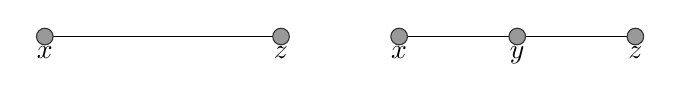
\begin{tikzpicture}[y=.3cm, x=.3cm,font=\normalsize]

\draw (0,0) -- (10,0);

\filldraw[fill=black!40,draw=black!80] (0,0) circle (3pt)    node[anchor=north] {$x$};
\filldraw[fill=black!40,draw=black!80] (10,0) circle (3pt)   node[anchor=north] {$z$};

\draw (15,0) -- (25,0);

\filldraw[fill=black!40,draw=black!80] (15,0) circle (3pt)   node[anchor=north] {$x$};
\filldraw[fill=black!40,draw=black!80] (25,0) circle (3pt)   node[anchor=north] {$z$};
\filldraw[fill=black!40,draw=black!80] (20,0) circle (3pt)   node[anchor=north] {$y$};
\end{tikzpicture}
\[\]

Hemos creado una subdivisión de la arista $xz$ en el camino $xyz$.
	
\begin{definition}
	Sea un grafo $G$ se dice completo si cada par de vértices $u$ y $v$ están conectados por una arista. Si el grafo $G$ completo tiene n vértices lo denominaremos $K_n$.
\end{definition}

\begin{definition}
	Un grafo $G$ se dice bipartito si su conjunto de vértices $V(G)$ es unión de dos subconjuntos disjuntos $V_1$ y $V_2$, de manera que las aristas del grafo conectan vértices $V_1$ y $V_2$ pero nunca    vértices de un mismo subconjunto ($V_1$ ó $V_2$). Es decir, existen $V_1,V_2 \subset V(G)$ cumpliendo:
	\begin{itemize}
		\item $V_1 \cup V_2 = V(G)$
		\item $V_1 \cap V_2 = \emptyset$
		\item $\forall v_{1},v_{2} \in V_j \hspace{0.1cm}  \hspace{0.1cm} \nexists e_{1},e_{2} \in E(G)$ tal que $e_{1}$ tenga como extremos a $v_{1}$ y $v_{2}$, $j=1,2$.
	\end{itemize}
\end{definition}

Ejemplo:

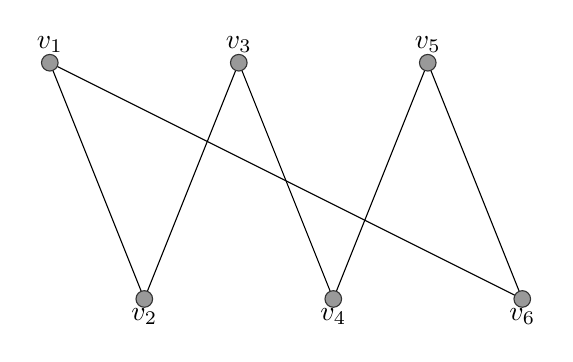
\begin{tikzpicture}[y=.3cm, x=.3cm,font=\normalsize]
	\draw (0,10) -- (4,0);
	\draw (0,10) -- (20,0);
	\draw (8,10) -- (4,0);
	\draw (8,10) -- (12,0);
	\draw (16,10) -- (12,0);
	\draw (16,10) -- (20,0);

	\filldraw[fill=black!40,draw=black!80] (0,10) circle (3pt)   node[anchor=south] {$v_1$};
	\filldraw[fill=black!40,draw=black!80] (8,10) circle (3pt)   node[anchor=south] {$v_3$};
	\filldraw[fill=black!40,draw=black!80] (16,10) circle (3pt)  node[anchor=south] {$v_5$};
	\filldraw[fill=black!40,draw=black!80] (4,0) circle (3pt)    node[anchor=north] {$v_2$};
	\filldraw[fill=black!40,draw=black!80] (12,0) circle (3pt)   node[anchor=north] {$v_4$};
	\filldraw[fill=black!40,draw=black!80] (20,0) circle (3pt)   node[anchor=north] {$v_6$};

\end{tikzpicture}

\begin{definition}
	Un grafo bipartito $G$ con  conjuntos de vértices destacados  $V_1$ y $V_2$ se dirá completo si  $\forall v_1 \in V_1 \text{,} \;\forall v_2 \in V_2 $, existe una arista que los conecta. Al grafo $G$ bipartito completo de n vértices en $V_1$ y m vértices en $V_2$ lo denominaremos $K_{n,m}$.
\end{definition}

Ejemplos de grafos completo ($K_5$), bipartito y bipartito completo ($K_{3,3}$):
	
\[\]
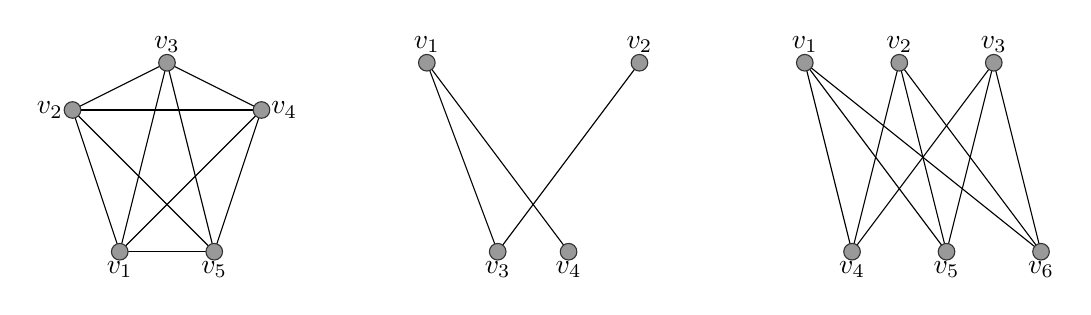
\begin{tikzpicture}[y=.3cm, x=.3cm,font=\normalsize]
\draw (2,0) -- (0,6);
\draw (2,0) -- (4,8);
\draw (2,0) -- (8,6);
\draw (2,0) -- (6,0);
\draw (0,6) -- (4,8);
\draw (0,6) -- (8,6);
\draw (0,6) -- (6,0);
\draw (4,8) -- (8,6);
\draw (4,8) -- (6,0);
\draw (8,6) -- (6,0);

\filldraw[fill=black!40,draw=black!80] (2,0) circle (3pt)    node[anchor=north] {$v_1$};
\filldraw[fill=black!40,draw=black!80] (0,6) circle (3pt)    node[anchor=east] {$v_2$};
\filldraw[fill=black!40,draw=black!80] (4,8) circle (3pt)    node[anchor=south] {$v_3$};
\filldraw[fill=black!40,draw=black!80] (8,6) circle (3pt)    node[anchor=west] {$v_4$};
\filldraw[fill=black!40,draw=black!80] (6,0) circle (3pt)    node[anchor=north] {$v_5$};

\draw (15,8) -- (18,0);
\draw (15,8) -- (21,0);
\draw (24,8) -- (18,0);

\filldraw[fill=black!40,draw=black!80] (15,8) circle (3pt)    node[anchor=south] {$v_1$};
\filldraw[fill=black!40,draw=black!80] (24,8) circle (3pt)    node[anchor=south] {$v_2$};
\filldraw[fill=black!40,draw=black!80] (18,0) circle (3pt)    node[anchor=north] {$v_3$};
\filldraw[fill=black!40,draw=black!80] (21,0) circle (3pt)    node[anchor=north] {$v_4$};

\draw (31,8) -- (33,0);
\draw (31,8) -- (37,0);
\draw (31,8) -- (41,0);
\draw (35,8) -- (33,0);
\draw (35,8) -- (37,0);
\draw (35,8) -- (41,0);
\draw (39,8) -- (33,0);
\draw (39,8) -- (37,0);
\draw (39,8) -- (41,0);

\filldraw[fill=black!40,draw=black!80] (31,8) circle (3pt)    node[anchor=south] {$v_1$};
\filldraw[fill=black!40,draw=black!80] (35,8) circle (3pt)    node[anchor=south] {$v_2$};
\filldraw[fill=black!40,draw=black!80] (39,8) circle (3pt)    node[anchor=south] {$v_3$};
\filldraw[fill=black!40,draw=black!80] (33,0) circle (3pt)    node[anchor=north] {$v_4$};
\filldraw[fill=black!40,draw=black!80] (37,0) circle (3pt)    node[anchor=north] {$v_5$};
\filldraw[fill=black!40,draw=black!80] (41,0) circle (3pt)    node[anchor=north] {$v_6$};
\end{tikzpicture}
\[\]

\begin{theorem}[\textbf{Teorema de Kuratowski}]
	Un grafo $G$ es plano si y sólo si no contiene ningún subgrafo que sea una subdivisión de $K_5$ ó $K_{3,3}$.
\end{theorem}
	
Por ejemplo: ¿El grafo $K_6$ es plano?
\[\]
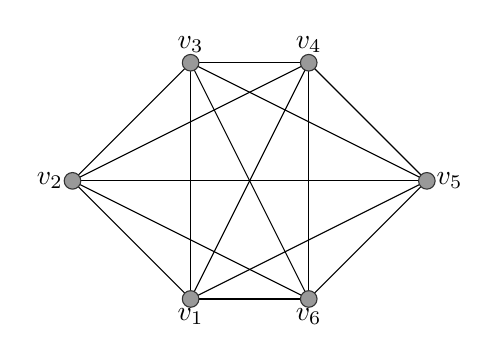
\begin{tikzpicture}[y=.3cm, x=.3cm,font=\normalsize]
\draw (15,0) -- (10,5);
\draw (15,0) -- (15,10);
\draw (15,0) -- (20,10);
\draw (15,0) -- (25,5);
\draw (15,0) -- (20,0);
\draw (10,5) -- (15,10);
\draw (10,5) -- (20,10);
\draw (10,5) -- (25,5);
\draw (10,5) -- (20,0);
\draw (15,10) -- (20,10);
\draw (15,10) -- (25,5);
\draw (15,10) -- (20,0);
\draw (20,10) -- (25,5);
\draw (20,10) -- (20,0);
\draw (25,5) -- (20,0);

\filldraw[fill=black!40,draw=black!80] (15,0) circle (3pt)    node[anchor=north] {$v_1$};
\filldraw[fill=black!40,draw=black!80] (10,5) circle (3pt)    node[anchor=east] {$v_2$};
\filldraw[fill=black!40,draw=black!80] (15,10) circle (3pt)    node[anchor=south] {$v_3$};
\filldraw[fill=black!40,draw=black!80] (20,10) circle (3pt)    node[anchor=south] {$v_4$};
\filldraw[fill=black!40,draw=black!80] (25,5) circle (3pt)    node[anchor=west] {$v_5$};
\filldraw[fill=black!40,draw=black!80] (20,0) circle (3pt)    node[anchor=north] {$v_6$};
\end{tikzpicture}
\[\]
	
	Por el teorema de Kuratowski, $K_{6}$ no es plano. En efecto, si eliminamos uno solo de sus vértices, y por ende las aristas que inciden sobre éste, obtenemos el grafo $K_5$.
	
	Una demostración muy simple y corta del teorema de Kuratowski se puede ver en \cite{Kuratowski}. No obstante nosotros sólo necesitaremos el hecho de que $K_{3,3}$ no es plano.
	Este resultado es la base de la demostración del teorema de la curva de Jordan y además no es complicado de demostrar, por lo tanto convendría pararse un momento para reflexionar sobre él. Para su demostración necesitamos el siguiente resultado.
	
\begin{lemma}
	Sea $C$ una curva poligonal de Jordan en el plano, entonces $\mathbb{R}^2 \backslash C$ tiene exactamente dos regiones con $C$ como frontera.
\end{lemma}

	A estas dos regiones las llamaremos interior y exterior de $C$ y las denotaremos por Int($C$) y Ext($C$) respectivamente. Además se tiene:
\[
\overline{Int(C)} = Int(C) \cup C
\]
\[
\overline{Ext(C)} = Ext(C) \cup C
\]

Ahora vamos a extender este resultado.

\begin{lemma}\label{lema24}
	Sea $C$ una curva poligonal simple y cerrada en el plano y $P$ un arco poligonal simple en $\overline{Ext(C)}$ tal que $P$ une $p$ y $q$ en $C$ y no tiene otros puntos en común con $C$. Sean $P_1$ y $P_2$ los dos arcos de $C$ con interiores disjuntos conectando $p$ a $q$: $C=P_1\cup P_2$, $P_1\cap P_2=\{p,q\}$. Entonces $\mathbb{R}^2 \backslash (C \cup P)$ tiene exactamente tres regiones con $C$,$P_{1} \cup P$ y $P_{2} \cup P$ como frontera, respectivamente.
	
El enunciado análogo es cierto si $P$ está contenido en  $\overline{Int(C)}$ y es disjunto con $C$ salvo sus extremos.
\end{lemma}

	Este lema implica que si $r$ y $s$ son puntos de $P_1 \backslash \{ p,q \}$ y $P_2 \backslash \{ p,q \}$, respectivamente, entonces no es posible unir $r$ con $s$  por arco poligonal simple en $\overline{Int(C)}$ sin cortar a $P$.

\begin{theorem}\label{lema25}
	$K_{3,3}$ no es plano.
\end{theorem}
\begin{proof}
Supongamos ahora que $K_{3,3}$ es  plano, y en virtud del lema \ref{lema22} entendámoslo dibujado en el plano de forma que sus aristas sean arcos poligonales simples. Llamemos como es habitual $V_1=\{v_1,v_2,v_3\}$ y $V_2=\{v_4,v_5,v_6\}$ a los dos conjuntos de vértices destacados de $K_{3,3}$.
Consideremos el ciclo poligonal $C_6$ en $\mathbb{R}^2$ definido sobre el dibujo embebido de  $K_{3,3}$  por los vértices $v_{1}v_{2}v_{3}v_{4}v_{5}v_{6}$. Destaquemos las aristas $v_{1}v_{4}$, $v_{2}v_{5}$ y $v_{3}v_{6}$ de $K_{3,3}$, obviamente disjuntas entre si y disjuntas con $C_6$,  salvo los vértices extremos contenidos en $C_6$. Claramente $C_6$ sería una curva poligonal de Jordan, y por el Lema anterior cada dos de las tres aristas destacadas han de estar contenidas en componentes conexas distintas de $\mathbb{R}^2\setminus C$ (excepto sus puntos extremos), ya que éstas no se cortan.  Esto contradice que $\mathbb{R}^2\setminus C$ tiene sólo dos componentes conexas.
\end{proof}

A continuación mostramos  los grafos que hemos usado en la demostración.

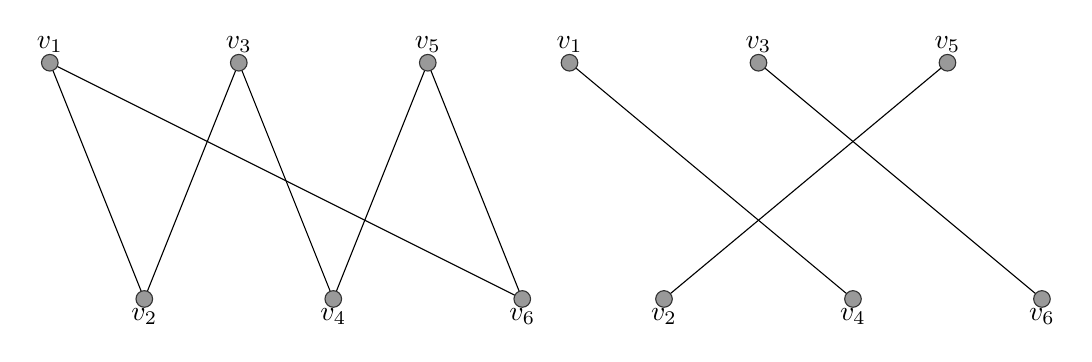
\begin{tikzpicture}[y=.3cm, x=0.3cm,font=\normalsize]
\draw (0,10) -- (4,0);
\draw (0,10) -- (20,0);
\draw (8,10) -- (4,0);
\draw (8,10) -- (12,0);
\draw (16,10) -- (12,0);
\draw (16,10) -- (20,0);

\filldraw[fill=black!40,draw=black!80] (0,10) circle (3pt)    node[anchor=south] {$v_1$};
\filldraw[fill=black!40,draw=black!80] (8,10) circle (3pt)    node[anchor=south] {$v_3$};
\filldraw[fill=black!40,draw=black!80] (16,10) circle (3pt)    node[anchor=south] {$v_5$};
\filldraw[fill=black!40,draw=black!80] (4,0) circle (3pt)    node[anchor=north] {$v_2$};
\filldraw[fill=black!40,draw=black!80] (12,0) circle (3pt)    node[anchor=north] {$v_4$};
\filldraw[fill=black!40,draw=black!80] (20,0) circle (3pt)    node[anchor=north] {$v_6$};

\draw (22,10) -- (34,0);
\draw (30,10) -- (42,0);
\draw (38,10) -- (26,0);

\filldraw[fill=black!40,draw=black!80] (22,10) circle (3pt)    node[anchor=south] {$v_1$};
\filldraw[fill=black!40,draw=black!80] (30,10) circle (3pt)    node[anchor=south] {$v_3$};
\filldraw[fill=black!40,draw=black!80] (38,10) circle (3pt)    node[anchor=south] {$v_5$};
\filldraw[fill=black!40,draw=black!80] (26,0) circle (3pt)    node[anchor=north] {$v_2$};
\filldraw[fill=black!40,draw=black!80] (34,0) circle (3pt)    node[anchor=north] {$v_4$};
\filldraw[fill=black!40,draw=black!80] (42,0) circle (3pt)    node[anchor=north] {$v_6$};
\end{tikzpicture}

Ahora ya estamos listos para llegar al objetivo de éste apartado: El teorema de la curva de Jordan.

\subsection{Teorema de la curva de Jordan: Demostración}

Para la demostración del teorema de la curva de Jordan necesitaremos, a parte del hecho ya enunciado de que $K_{3,3}$ no es plano, dos resultados que nos serán de utilidad.

\begin{lemma}\label{proposicion26}
	Si $C$ es una curva de Jordan, entonces $\mathbb{R}^{2} \backslash C$ es disconexo.
\end{lemma}
	
\begin{proposition}\label{proposicion211}
	Si $P$ es un arco de poligonal simple en el plano, entonces $\mathbb{R}^2 \backslash P$ es conexo.
\end{proposition}

\begin{definition}
	Sea $C$ un subconjunto cerrado del plano y $\Omega$ una región de $\mathbb{R}^2 \backslash C$. Un punto $p \in C$ es accesible desde $\Omega$ si para algún (y por lo tanto para cada) punto $q \in \Omega$ existe un arco poligonal simple de $q$ a $p$ teniendo sólo el punto $p$ en común con $C$.
\end{definition}

Si $C$ es una curva de Jordan, $p\in C$ y $\Omega$ es una región de  $\mathbb{R}^2 \backslash C$,  no está claro que $p$ tenga que ser accesible desde $\Omega$. Sin embargo, tenemos el siguiente resultado.

\begin{lemma}
Si $C$ es una curva de Jordan en el plano y $\Omega$ es una región de  $\mathbb{R}^2 \backslash C$, el conjunto de puntos de $C$  accesibles desde $\Omega$  es denso en $C$.
\end{lemma}
\begin{proof} En efecto, si $P$ es cualquier arco de $C$ que contiene a $p\in C$, entonces la proposición \ref{proposicion211} implica que $\mathbb{R}^2 \backslash (\overline{C \backslash P})$ es conexo y por tanto contiene un arco poligonal simple $P'$ conectando $p$ con un punto  $q$ de cualquiera región de $\mathbb{R}^2 \backslash C$ distinta de $\Omega$ (que sabemos existe ya que $\mathbb{R}^2 \backslash C$  es disconexo). Necesariamente  $P'$ ha de cortar a $C$ en algún punto de $P$ que será accesible desde $\Omega$, y como $P$ puede ser  arbitrariamente pequeño  concluimos que los puntos de $C$ accesibles desde $\Omega$ son densos en $C$. 
\end{proof}
Una consecuencia inmediata de este lema es que si $C$ es una curva Jordan  en el plano, $C$ es la frontera de cualquiera de las componentes conexas de $\mathbb{R}^2\setminus C$.
Podemos ahora demostrar el teorema buscado.

\begin{theorem}[\textbf{Teorema de la curva de Jordan}]
	Sea $C$ una curva de Jordan $\Rightarrow$ $\mathbb{R}^2 \backslash C$ tiene exactamente dos regiones, ambas con $C$ como frontera.
\end{theorem}

\begin{proof}
Realizaremos ésta demostración por reducción al absurdo, y asumamos oor el Lema \ref{proposicion26}  que $\mathbb{R}^2 \backslash C$ tiene más de dos componentes conexas. Fijemos  tres componentes conexas distintas $\Omega_1$, $\Omega_2$ y $\Omega_3$ de $\mathbb{R}^2 \backslash C$ y elijamos $q_j\in \Omega_j$, $j=1,2,3$.
Sean $Q_1$, $Q_2$, $Q_3$ subarcos disjuntos dos a dos de $C$. 	 Por el lema anterior, $Q_j$ contiene puntos accesibles desde $\Omega_i$, por lo que $\Omega_i$ contiene un arco poligonal simple $P_{i,j}$ con punto inicial $q_i$ y final en un punto de $Q_j$,  $\forall i,j =$ 1, 2, 3. Salvo rectificar el dibujo de los arcos, podemos asumir que $P_{i,j} \cap P_{i,j'} = {q_i}$ $j \neq j'$. Además es claro que $P_{i,j} \cap P_{i',j'} = \emptyset$ por estar en regiones distintas de $\mathbb{R}^2 \backslash C$.
Añadiendo a los arcos $P_{i,j}$ convenientes trozos de arco  dibujados sobre $C$,  los arcos de Jordan resultantes (también denotados $P_{i,j}$) definen un grafo plano isomorfo a $K_{3,3}$, lo que contradice el Teorema \ref{lema25}.

Por tanto, $\mathbb{R}^2 \backslash C$ tiene exactamente dos regiones,  que llamaremos  $Ext(C)$ (no acotada) e $Int(C)$ (acotada), con frontera común $C$.
\end{proof}

Como nota final, sólo decir que el teorema de la curva de Jordan es un caso particular del teorema de Jordan-Schönflies que enunciaremos en la siguiente sección.

\section{Teorema de Jordan-Schönflies}

En ésta segunda sección vamos a comentar algunas implicaciones topológicas del teorema de Jordan-Schönflies, una generalización fuerte del teorema de la curva de Jordan. Este resultado  se enunciará si demostración y que su tratamiento excede el ámbito de este trabajo. 
Comenzaremos extendiendo el lema \ref{lema24}:

\begin{lemma}
	Sea $C$ una curva de Jordan y $P$ un arco   simple en $Int(C)$ tal que $P$ una $p,q \in C$ y no tiene otro punto en común con $C$. Sean $P_1$ y $P_2$ los dos arcos en $C$ que unen $p$ y $q$. Entonces $\mathbb{R}^2 \backslash (C \cup P)$ tiene exactamente tres regiones cuyas fronteras son $C$, $P\cup P_1$ y $P\cup P_2$, respectivamente.
\end{lemma}

	La generalización que se ha hecho en éste lema es que hemos pasado de poligonales simples cerradas a curvas de Jordan.
	
	\begin{definition}
Si $S$ es un conjunto, entonces $\vert S \vert$ denotará su cardinal.
\end{definition}
El siguiente resultado, corolario inductivo de lema anterior, simplemente expresa que la característica de Euler de la esfera es $2$:
\begin{lemma}
	Si $\Gamma$ es un grafo plano biconexo conteniendo un ciclo $C$ (que de hecho es una curva de Jordan) tal que todas aristas de $\Gamma \backslash C$ son arcos simples en $\overline{Int(C)}$. Entonces $\mathbb{R}^2 \backslash \Gamma$ tiene exactamente $\vert E(\Gamma) \vert - \vert V(\Gamma) \vert + 2$ regiones (llamadas caras de $\Gamma$). Cada una de ellas con un ciclo de $\Gamma$ como frontera.
\end{lemma}

Un uso elaborado del anterior lema  permite demostrar el siguiente resultado, uno de los pilares fundamentales de la Topología plana.

\begin{theorem}[\textbf{Teorema de Jordan-Schönflies}]
	Sea $f$ un homeomorfismo de una curva de Jordan $C$ en otra curva curva de Jordan $C'$. Entonces $f$ puede ser extendido a un homeorfismo $F$ de todo el plano.
\end{theorem}
 

\begin{definition}
	Sea $F$ un conjunto cerrado del plano, decimos que un punto $p \in F$ es curvo-accesible si, para cada punto $q$ que no esté en $F$, existe un arco simple de $q$ a $p$ que sólo tenga $p$ en común con F.
\end{definition}

Como trivialmente todo punto de $\mathbb{S}^1$ es curvo accesible, el teorema de Jordan-Schönflies implica que que todo punto en una curva de Jordan es curvo-accesible. Como consecuencia, y usando el círculo de ideas alrededor del teorema de la curva de Jordan, es posible demostrar el siguiente:

\begin{theorem}
	Sea $F$ un conjunto cerrado en el plano con, al menos, tres puntos curvo-accesibles, entonces $\mathbb{R}^2 / F$ tiene como máximo dos regiones.
\end{theorem}

\begin{definition}
	Si $C$ y $C'$ son curvas de Jordan y $\Gamma$ y $\Gamma'$ son grafos biconexos que consisten en $C$ (respectivamente $C'$) y arcos   simples en $\overline{Int}(C)$ (respectivamente $\overline{Int}(C')$), entonces $\Gamma$ y $\Gamma'$ se dice que son plano-isomorfos si existe un isomorfismo de $\Gamma$ en $\Gamma'$ cumpliendo 
\begin{enumerate}
	\item Un ciclo en $\Gamma$ es la frontera de una cara de $\Gamma$     $\iff$ La imagen del ciclo por el isomorfismo es la frontera de una cara de $\Gamma'$.
	\item La imagen por el isomorfismo del ciclo exterior de $\Gamma$ (véase $C$) es el ciclo exterior de $\Gamma'$ (véase $C'$).
\end{enumerate}	
\end{definition}
El teorema de Jordan-Schönflies admite la siguiente generalización:
\begin{theorem}\label{teorema33}
	Sean $\Gamma$ y $\Gamma'$ grafos planos biconexos tales que $g$ sea un homeomorfismo y un plano-isomorfismo de $\Gamma$ en $\Gamma'$. Entonces $g$ puede ser extendido a un homeomorfismo de todo el plano.
\end{theorem}

\begin{proof}
	Esta demostración la haremos por inducción sobre el número de aristas de $\Gamma$.

	Si $\Gamma$ es un ciclo, entonces el problema se reduce al teorema de Jordan-Schönflies. De otro modo se sigue del lema \ref{lema27} que $\Gamma$ tiene un camino $P$ y un subgrafo biconexo $\Gamma_1$ que contiene al ciclo exterior de $\Gamma$, de tal modo que $\Gamma$ se obtiene a partir de $\Gamma_1$ añadiéndole $P$ en $\overline{Int}(C)$, donde $C$ es la frontera de una de las caras de $\Gamma_1$.

	Ahora aplicamos la hipótesis de inducción a $\Gamma_1$ y después a los dos ciclos de $C \cup P$ conteniendo a $P$.
\end{proof}
